\documentclass[tikz,border=2pt]{standalone}
\usepackage{graphicx}
\usepackage{xcolor}
\usetikzlibrary{arrows.meta}
\begin{document}
\begin{tikzpicture}[x=1cm,y=1cm,>=Latex]
  % Exact Figure 1 artwork recovered from the submitted PDF.
  \node[anchor=south west,inner sep=0] (fig) at (0,0.34)
    {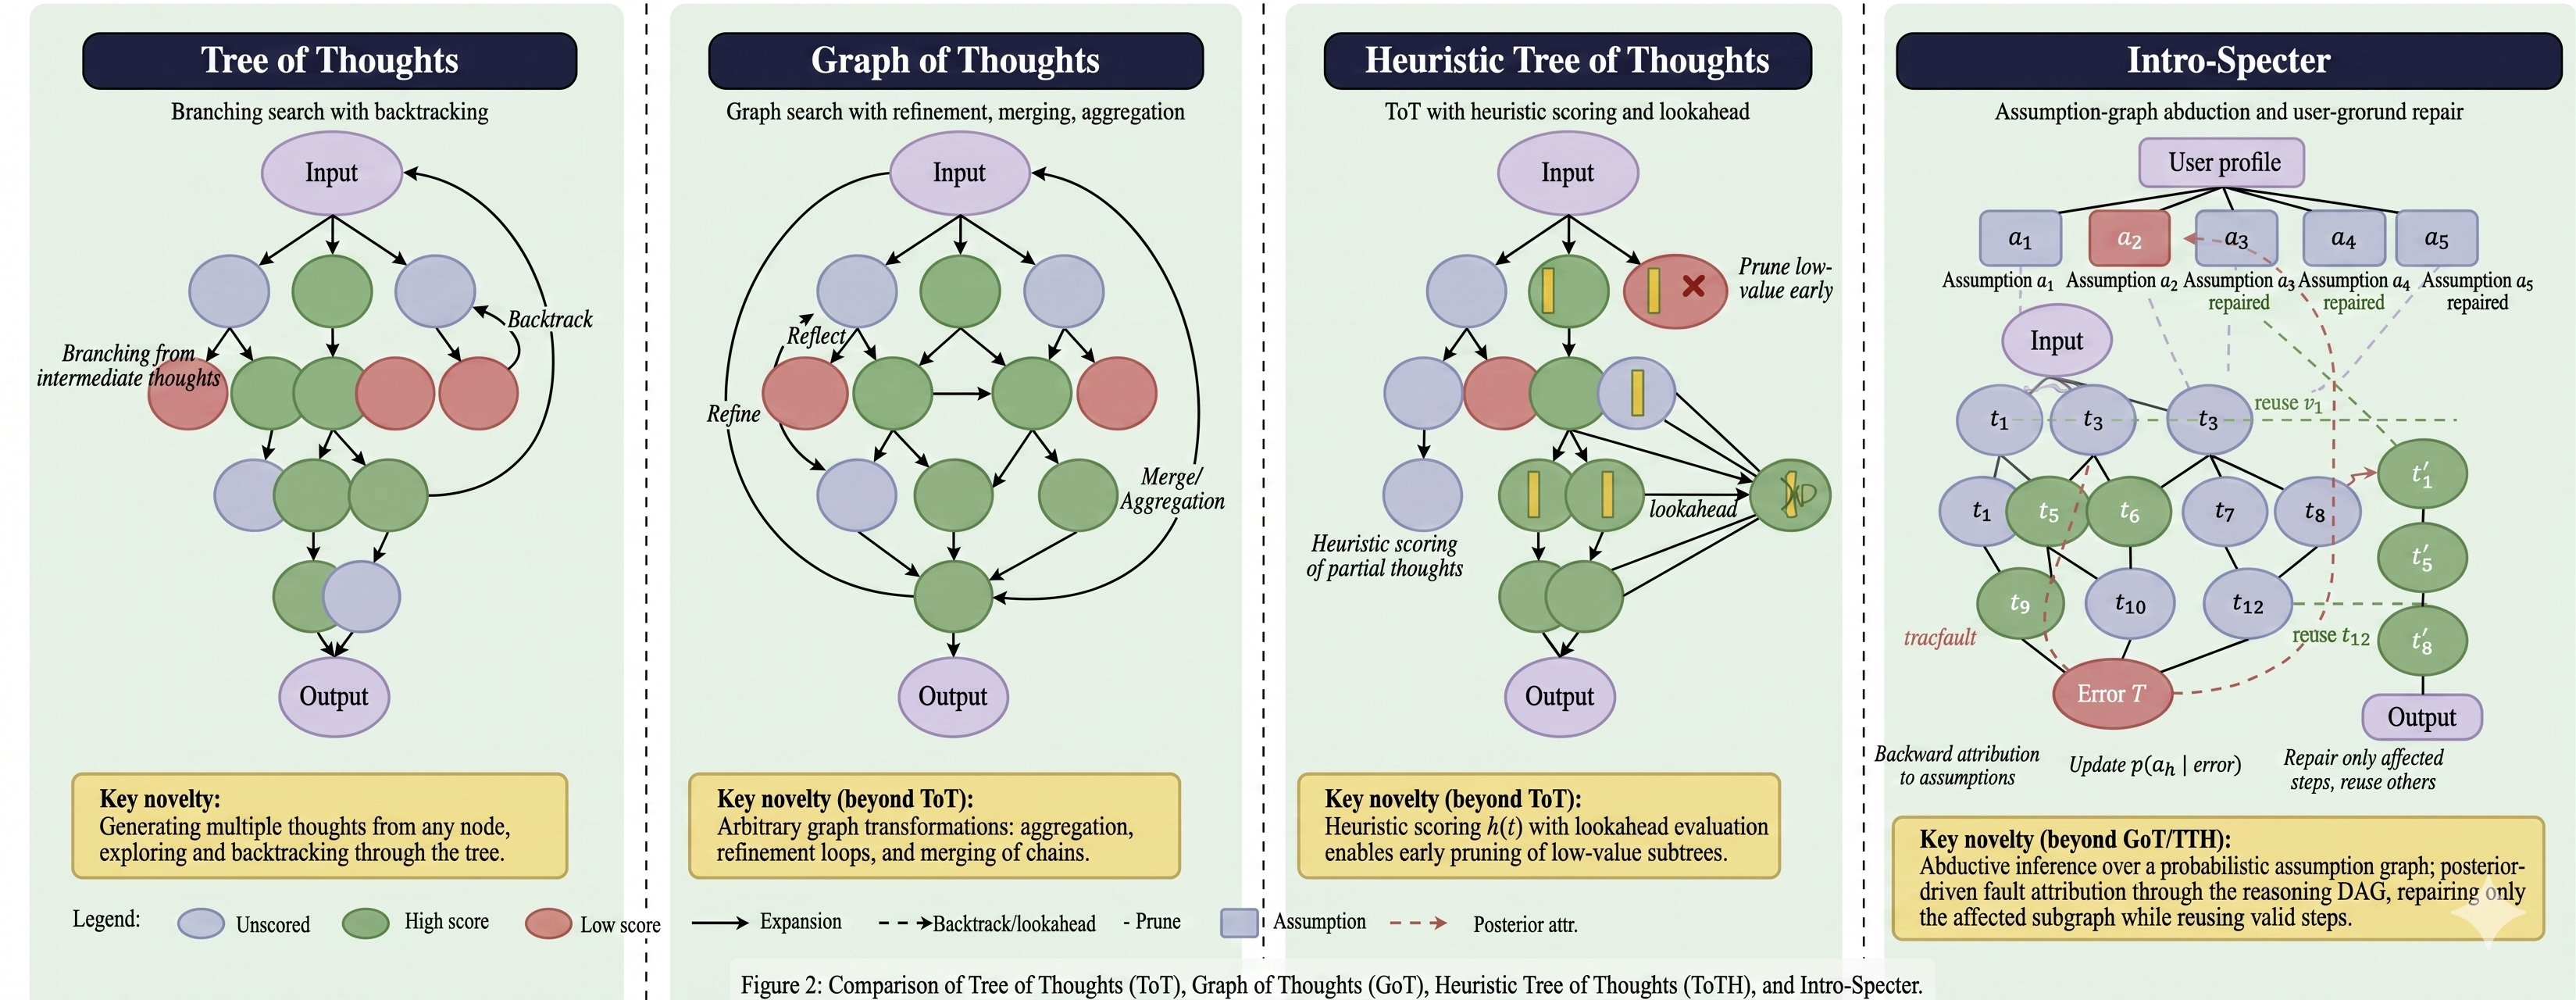
\includegraphics[width=17cm]{figure2_comparison_original.jpg}};

  % Explicit line-style legend requested for the redraw.
  \draw[->,black,line width=.65pt] (5.05,0.16) -- (6.05,0.16);
  \node[anchor=west,font=\sffamily\scriptsize] at (6.15,0.16) {dependency edge};
  \draw[->,red!70!black,dashed,line width=.9pt] (9.0,0.16) -- (10.0,0.16);
  \node[anchor=west,font=\sffamily\scriptsize] at (10.10,0.16) {counterfactual attribution};
\end{tikzpicture}
\end{document}
